% !TeX root = RJwrapper.tex
\title{crsra: A package for Cleaning and Analyzing Coursera Research Export
Data}
\author{by Aboozar Hadavand, Jeffrey Leek}

\maketitle

\abstract{%
An abstract of less than 150 words.
}

\subsection{Introduction}\label{introduction}

It is hard to pin down the time of the birth of the first Massive Open
Online Course
(MOOC).\footnote{Some have claimed Sesame Street as the first MOOC. Delaney Parrish, "Sesame Street was the original MOOC," *BROOKINGS NOW*, The Brookings Institution, June 18, 2015, https://www.brookings.edu/blog/brookings-now/2015/06/18/sesame-street-was-the-original-mooc/}
But since the advent of more focused MOOCs pioneered by universities and
platforms such as Coursera, Udacity, and edX, reserachers have tried to
focus on studying MOOCs. There are fundamental differences between
traditional education and MOOCs was large enough to attract reserachers
to study students' behavior and outcomes. These differences are best
reflected in the definition of MOOCs by \cite{mcauley2010mooc} that
``{[}a{]}n online course with the option of free and open registration,
a publicly shared curriculum, and open-ended outcomes which integrates
social networking, accessible online resources \ldots{} and most
significantly builds on the engagement of learners who self-organize
their participation according to learning goals, prior knowledge and
skills, and common interests.''

Research on MOOCs few years with more data being accumulated and
collected. \cite{bozkurt2017trends} studied literature published on
MOOCs throught 2015 and found that the number of articles published on
the subject increased from 1 in 2008 to 170 in 2015. More research in
needed to fully understand the effectiveness, reach, limits, and the
potential of MOOCs. However, one of the main challenges in studying
MOOCs remains to be data. Data is not usually publically available since
it is owened by private MOOC providers and there are concerns about
privacy of students. More importantly, as \cite{lopez2017google} point
out, the size and complexity of MOOC data is an overwhelming challenge
to many researchers. Therefore, it is imperative to provide tools that
pave the way for more research on the new subject of MOOCs.

This paper introduces a package called \emph{crsra} based on the
statistical sofware R to help clean and analyze large loads of data from
the Coursera MOOCs. The advantages of the package are as follows: a)
faster loading of data for analysis, b) efficient method for combining
data from multiple courses and even across
institutions,\footnote{This is important since although MOOC researchers have access to thousands of students in their sample, few studies benefit from data across multiple courses and institutions. Such analysis helps draw more robust conclusions about student behaviors \citep{reich2015rebooting}.}
and c) provision of a set of functions for analysing student behaviors.

\subsection{Coursera Research Data}\label{coursera-research-data}

Coursera is one of the main providers of MOOCs that launched in January
2012. In fact, with over 25 million learners, Coursera is the biggest
provider in the world being followed by EdX, the MOOC provider that was
a result of a collaboration between Harvard Universit and MIT, with over
10 million users. Coursera has over 150 uiveristy partners from 29
countries and offers a toatl of 2000+ courses from computer science to
philosophy \citep{coursera}. In addition, Coursera offers 180+
specialization, Coursera's own credential system, and 4 fully online
Masters degrees. Courses include recorded video lectures, graded
assignment, quizzes, and discussion forums.

Since the early years of the platform, Coursera has encouraged
researchers to analyze students' data and has facilitated the use of the
data and the platform for A/B testing. Starting November 2015 Coursera
introduced a dashboard for self-service data exports. Through this tool,
partner institutions and instructors can download data for a single
course or all courses associated with the institutuion. Research data
exports are sets of CSV files and are designed for use in relational
database systems. One of the advantages of the data is the existence of
a single \emph{hashed user ID} for each student. This user ID is
consistent for learners across all courses offered by an individual
institution and allows for connecting learner grades and progress across
course.

There are five types of research data export for each course. The Table
\ref{tab:datatypes} summarizes these five types. This set of data is
written in roughly 100 tables: some containing course information and
content, some containing students' information, progress, and outcomes,
and some containing forum data. Figure \ref{figure:datatables} shows

\begin{table}
\footnotesize
\caption{Types of research data export}\
\centering
\label{tab:datatypes}
\begin{tabular}{p{4cm}|p{7cm}}
Data Type & Description \\
\addlinespace
\toprule
Assessment submission data & Assessment submissions of quizzes, peer review, and programming assignments by learners.\\
\midrule
Course grade data & Contains the highest grade achieved by each learner on each required assessment as well as the timestamp of the learner's highest-scoring submission. This table also includes each learner's overall grade in the course.\\
\midrule
Course progress data & Contains data data documenting the timestamp for when the learner interacted with each piece of course content and the timestamps for when items were opened, completed, reopened, reattempted, etc.\\
\midrule
Demographic data & Contains the following information for all enrolled learners: general geographical data (based on IP address), browser language preference, and information for learners who completed their learner profile responses or participated in Coursera's platform-wide demographic survey (including age, gender, education level, and employment status).\\
\midrule
Discussion data & Contains forum activity data such as posts, responses, upvotes/downvotes, flags, and questions and answers associated with course content items.\\
\addlinespace
\bottomrule
\end{tabular}
\end{table}

\begin{figure}[htbp]
    \centering
    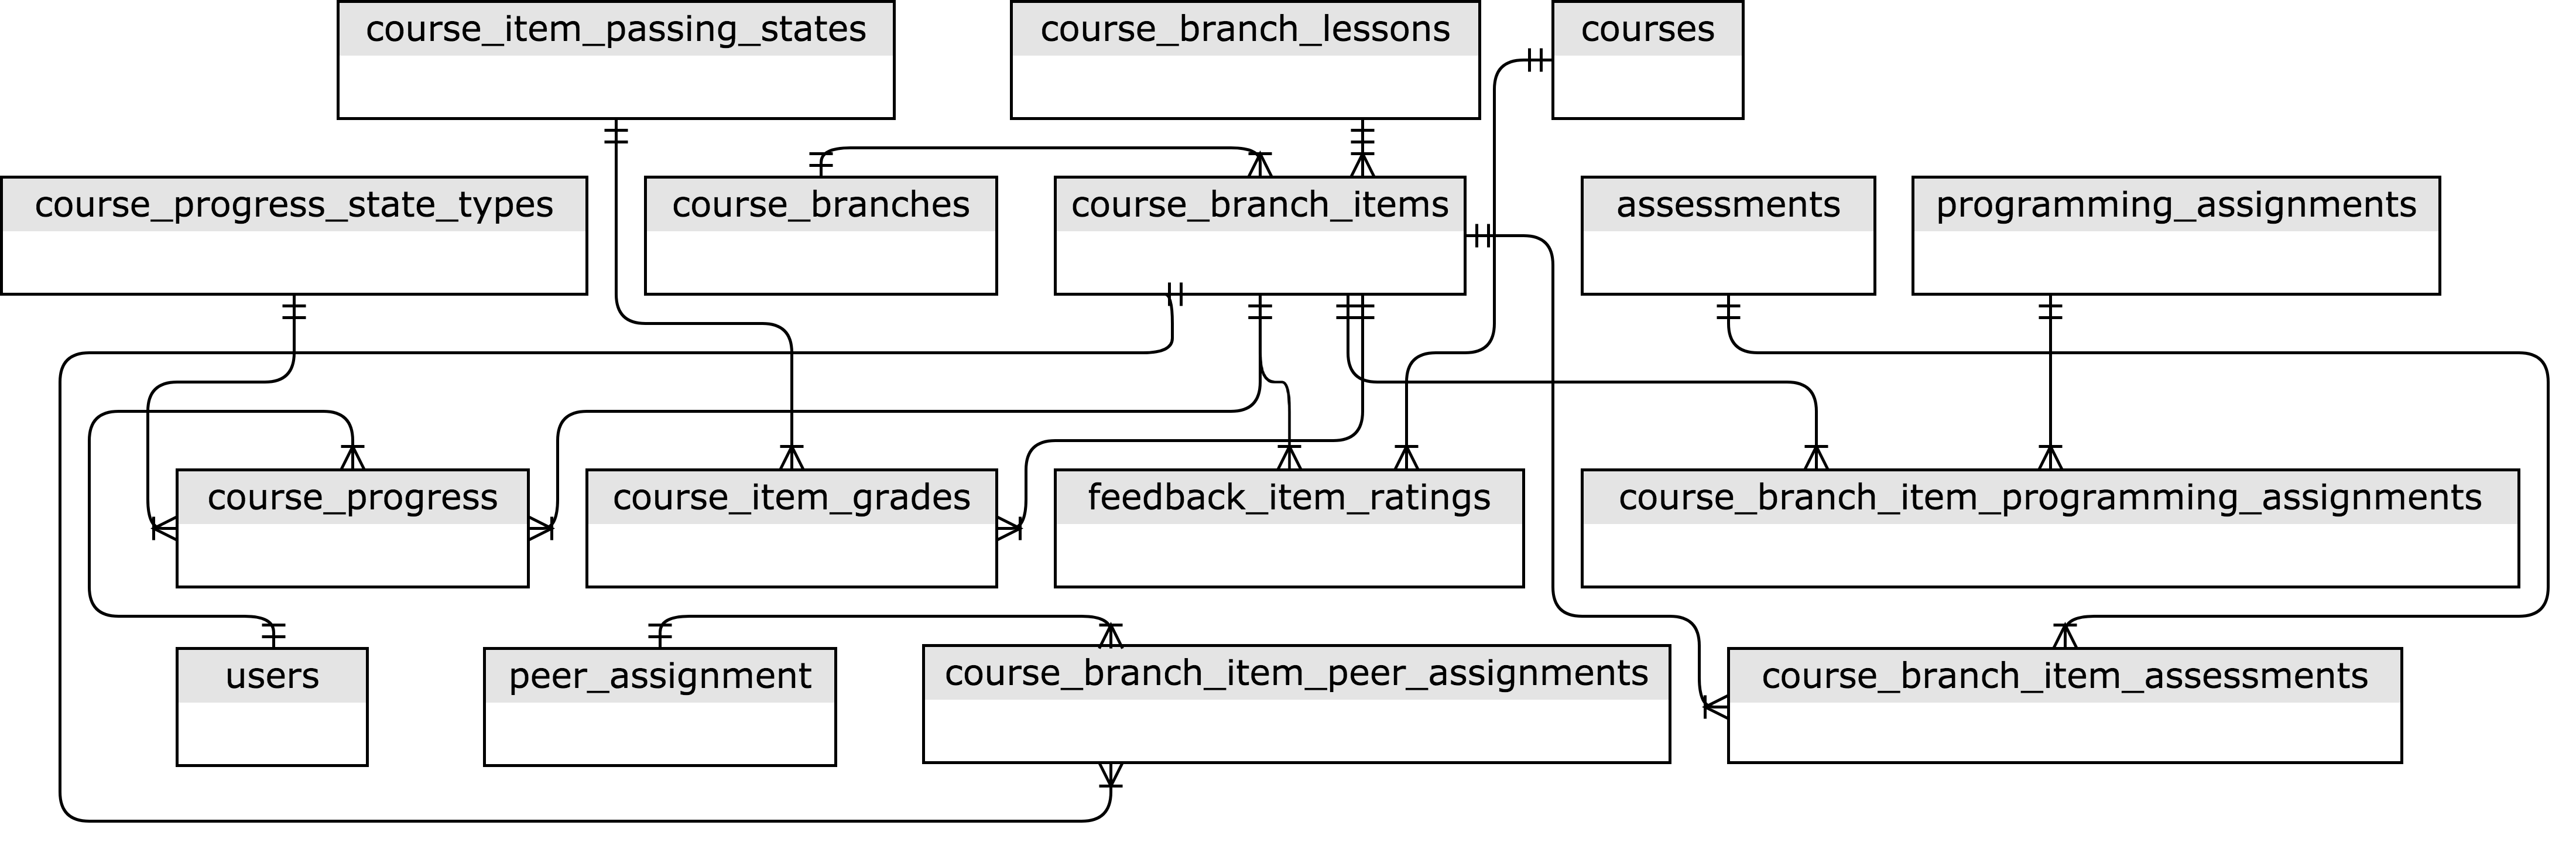
\includegraphics[scale=0.5]{datatables}
    \caption{The major relationships between tables groups, with minor connections omitted (Source: Coursera)}
    \label{figure:datatables}
\end{figure}

While Coursera provides tools for creating Postgres databases in a
docker
container\footnote{The tools is called `courseraresearchexports` and can be found here: https://github.com/coursera/courseraresearchexports},
as we mentioned earlier, importing data for analysis remains to be a
challenge for researchers with limited experience with relational
databases. Moreover, such tools are usually not platform
independent.\footnote{In an initial version of *crsra* based on Postgresql we had the problem of some team members not being able to set up the database properly on their PCs.}

\subsection{\texorpdfstring{The \emph{crsra}
Package}{The crsra Package}}\label{the-crsra-package}

The \emph{crsra} package helps import and organize Coursera's research
data exports into R. It also run some preliminary analysis on the data.
In the following section, we introduce the package and provide
instruction on how to import Coursera research data exports. To install
this package, you will need to install \emph{devtools}. Install the
\href{https://CRAN.R-project.org/package=devtools}{devtools package},
available from CRAN. Then execute the following commands to install the
\emph{crsra} package

\begin{Schunk}
\begin{Sinput}
library("devtools")
devtools::install_github("jhudsl/crsra", build_vignettes = TRUE)
\end{Sinput}
\end{Schunk}

In order to import your data dump into R, first point your working
directory to the directory that contains all the unzipped course
folders. Then execute the command \texttt{crsra\_import()}. If you are
not pointing to the correct directory, you will receive a warning and
the execution will be halted. Note that the data import may take some
time if the course data is large and there are several courses in your
working directory. Also note that by running the
\texttt{crsra\_import()} command, you import all tables for each
individual course into R in a list called \texttt{all\_tables}.

For a list of all the tables in the data download, please click
\href{https://github.com/jhudsl/crsra/blob/master/ListofTables.md}{here}.
All tables can be called using
\texttt{all\_tables{[}{[}"course\_name"{]}{]}{[}{[}"table\_name"{]}{]}}.
For instance, if you like to call the table \texttt{peer\_comments} in
the course Regression Models, you can simply execulte
\texttt{all\_tables{[}{[}"Regression\ Models"{]}{]}{[}{[}"peer\_comments"{]}{]}}.
To see a list of courses imported by the \texttt{crsra\_import()}
command check the variable \texttt{coursenames}. To see a list of all
the tables check the variable \texttt{tablenames}.

To see the data import in use, we use the package on data from Johns
Hopkins University (JHU) Data Science Specialization on Coursera. This
specialization, developed by Jeffrey Leek, Roger Peng, and Brian Caffo,
consists of ten courses. There has been more than two million
enrollments since the launch of this program in April 2014. The size of
data on the students who took these ten courses since 2015 is around 18
gigabytes. We used the \emph{crsra} package to import the data on all
the courses and then to find the number of students who passed a
specific course item (course item \texttt{67c1O}) in the course
``Regression Models'' and their average grade in a specific course.

\begin{Schunk}
\begin{Sinput}
library(dplyr)

all_tables[["Regression Models"]][["course_item_grades"]] %>%
    dplyr::filter(course_item_id == "67c1O") %>% 
    dplyr::filter(course_item_passing_state_id == 2) %>% 
    dplyr::summarise(n = n(), grade = mean(course_item_grade_verified))

## A tibble: 1 x 2
##      n     grade
##   <int>    <dbl>
## 1  8640 0.9556052
\end{Sinput}
\end{Schunk}

The package also includes a few other functions are added to the package
in addition to the main \texttt{crsra\_import()} function. A list of
functions and their descriptions is provided in Table
\ref{tab:functions}.

\begin{table}
\footnotesize
\caption{Other functions in the *crsra* package}\
\centering
\label{tab:functions}
\begin{tabular}{p{3cm}|p{7cm}}
Function & Description \\
\addlinespace
\toprule
\texttt{crsra\_membershares} & Returns a summary of the total number and the shares of users in each course broken down by factors such as roles, country, language, gender, employment status, education level, and student status.\\
\midrule
\texttt{crsra\_gradesummary} & Returns total grade summary or broken down by the factors mentioned above.\\
\midrule
\texttt{crsra\_progress} & Summarizes, for each course item, the total number and the share of users who stopped the course at that specific course item. The function ranks course items by their attrition.\\
\midrule
\texttt{crsra\_assessmentskips} & Users may "skip" reviewing a submission if there is a problem with it. This function categorizes skips by their type such as "inappropriate content", "plagiarism", etc. The function also returns list of mostly used words in peer comments.\\
\midrule
\texttt{crsra\_timetofinish} & Calculates the time to finish a course for each user.\\
\addlinespace
\bottomrule
\end{tabular}
\end{table}

\subsection{use another example given the functions
above}\label{use-another-example-given-the-functions-above}

\subsection{A Preliminary Analysis of Student Behavior on
Coursera}\label{a-preliminary-analysis-of-student-behavior-on-coursera}

Understanding how students progress through an education program is
critical for any educational planning and decision making
\citep{king1972primary}. Models of student progress are needed in order
to estimate the probability of a student completing a certain item in a
course and predict the time required to finish a course. Furthermore,
common measures of academic success and progres cannot be defined in the
same way for MOOCs. For instance, as \cite{perna2014moving} states, we
have limited knowledge on whether learners' progress through a MOOC
should be measured in a sequential fashion or in a way that captures the
flexibility and freedom in learning behavior that is unique to MOOCs.

We have limited understanding of user progress in MOOCs. There are only
a handful of studies on the subject of student pace, who completes
classes, and learning sequence in MOOCs. \cite{perna2014moving} perform
a descriptive analysis of student progress throught a set of 16 courses
on Coursera. They find that most users accessed course content in the
sequential order defined by the instructor of the course.
\cite{ho2014harvardx} study 17 courses taught on EdX and find that most
of the attrition in courses happen in the first week of course activity
(about 50 percent attrition) and that the avergae percentage of learners
who cease activity in the second week declines shaprty to 16 percent.
Most of these studies are specific to a set of courses or platforms. Due
to the many differences in the characteristics of MOOCs, any
extrapolation of the results to MOOCs in general has to be done with
caution.

In the following section, we will investigate students' progress through
the ten Data Science Specialization courses on Coursera provided by JHU.
Using the \texttt{crsra\_timetofinish} function in the \emph{crsra}
package, we can first investigate the time difference ebtween the first
and last activities within a course for each student. Time to finish is
only calculated for those who finished the course. Figure
\ref{figure:timetofinish} depicts the density function for time to
finish for three of the courses in the specialization. Note that the
density functions vary across courses. While for \emph{Developing Data
Products} and \emph{Getting and Cleaning Data} a majority of students
finish the courses in around 30 days, for \emph{Data Science Capstone} a
majority of students finish the course in 50 days.

\begin{Schunk}
\begin{Sinput}
TTF <- crsra_timetofinish()
\end{Sinput}
\end{Schunk}

\begin{figure}[htbp]
    \centering
    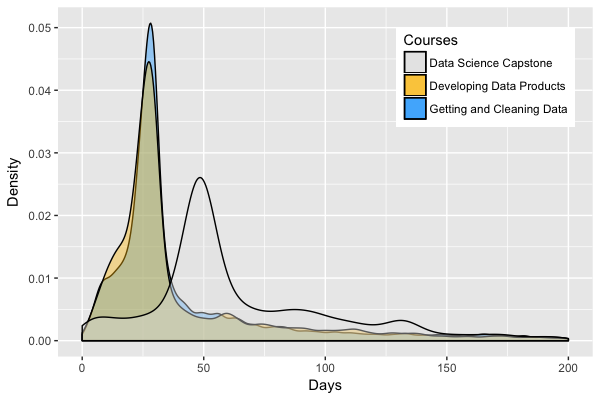
\includegraphics[scale=0.5]{timetofinish}
    \caption{Density functions for time to finish defined as the time difference between the first and last activities across three courses}
    \label{figure:timetofinish}
\end{figure}

In the table called \texttt{users}, Coursera provides a field for
student status of the learner including full-time and par-time students
and those who are not degree students. We can look at how time to finish
is different for groups with different student status. Figure
\ref{figure:stustatus} reports this for the course \emph{Getting and
Cleaning Data} and shows that part-time students take longer to finish
the course.

\begin{Schunk}
\begin{Sinput}
TTF.Status <- TTF[["Getting and Cleaning Data"]] %>% 
    dplyr::left_join(all_tables[["Getting and Cleaning Data"]][["users"]], 
                     by = "jhu_user_id", `copy`=TRUE) %>% 
    dplyr::filter(!is.na(student_status))
\end{Sinput}
\end{Schunk}

\begin{figure}[htbp]
    \centering
    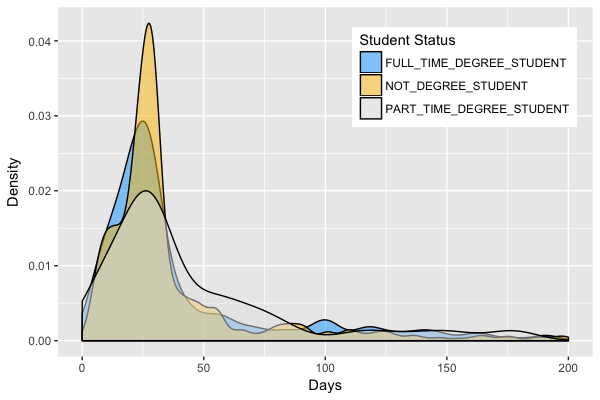
\includegraphics[scale=0.5]{stustatus}
    \caption{Density functions for time to finish across groups with different student statuses through the course Getting and Cleaning Data}
    \label{figure:stustatus}
\end{figure}

Our next step is to understand student progress in the courses. One of
the factors that distinguishes MOOCs from traditional classrooms is the
flexibility in advancing through the course. While in traditional
education the class length, pace, and completion dates are determined by
instructor of the course, in MOOCs it is the student who, for the most
part, has the freedom to choose these factors. This is evident by
looking at the time gap between completing each item in the course. We
can first look at how many course items students pass in the first week
of course activity. One obvious but yet interesting finding is large
variations across students. For instance, if we look at the course
\emph{Getting and Cleaning Data}, we can use the following code to find
the number of course items completed in the first week of course
activity. The course has roughly 40 items including lectures and
assignments. The variable \texttt{nweek1} captures the number of passed
course items in the first week of course activity, calculated as one
week after the first activity in the class. The density function in
Figure \ref{figure:passeditems} represents the variations across
students. For a majority of learners, the number of passed course items
in the first week is two. However, the number of those who finish mor
than 10 items in the first course is significant. Also interesting is
the double-peak shape of the density function. It is intersting to see
that there are more people who complete 12 course items in the first
week than there are who complete 7 course items. This indicates an
intersting structural change in students' pace between course items 7
and 12.

\begin{Schunk}
\begin{Sinput}
passed.items <- all_tables[["Getting and Cleaning Data"]][["course_progress"]] %>%
    dplyr::group_by(jhu_user_id) %>%
    # 604800 is the number of seconds in a week
    dplyr::filter(course_progress_ts <= min(course_progress_ts) + 604800) %>% 
    dplyr::summarise(nweek1 = n())
\end{Sinput}
\end{Schunk}

\begin{figure}[htbp]
    \centering
    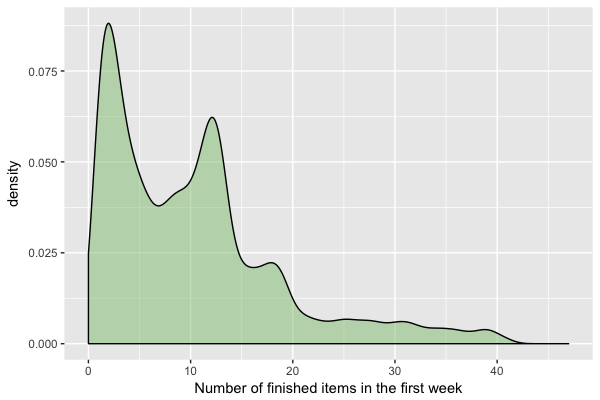
\includegraphics[scale=0.5]{passeditems}
    \caption{Density functions for the number of passed items in the first week of course activity for Getting and Cleaning Data}
    \label{figure:passeditems}
\end{figure}

A third interesting variable to look at when studying students' progress
in MOOCs is the time gaps between each session. In this exercise, we
looked at the time lapsed between each two consecutive course items for
each learner throughout the course \emph{Getting and Cleaning Data}. We
used the following code for the analysis. Note that we have ranked
course itmes based on the timestamp when student passes them and not
their natural order defined by the course instuctor.

\begin{Schunk}
\begin{Sinput}
gaps <- all_tables[["Getting and Cleaning Data"]][["course_progress"]] %>%
    # 2 is an indicator that the course item is completed
    dplyr::filter(course_progress_state_type_id == 2) %>% 
    dplyr::group_by(jhu_user_id, course_item_id) %>%
    # This is for keeping only the latest event for each course item
    dplyr::filter(course_progress_ts == max(course_progress_ts)) %>%
    dplyr::ungroup() %>%
    dplyr::arrange(jhu_user_id, course_progress_ts) %>%
    dplyr::group_by(jhu_user_id) %>%
    # This is for converting the time gap to hours
    dplyr::mutate(time.dif = as.numeric(course_progress_ts - 
                                            lag(course_progress_ts))/3600) %>%
    dplyr::filter(!is.na(time.dif)) %>% 
    dplyr::filter(time.dif != Inf | time.dif != -Inf)
\end{Sinput}
\end{Schunk}

Figure \ref{figure:sampleprogress} shows student progress in the course
Getting and Cleaning Data for three sample students. The vertical axis
is the gap between two consecutive sessions in hours. These three
students are chosen intentionally to show three different learning
paths. Panel A shows progress for a student with short gaps between
sessions for the first half of the course and longer gaps towards the
end. For future reference we call this pattern ``slowing down'' pattern.
This pattern is typical of many students in this course. Panel B shows
progress for a student with short gaps between sessions in the begining
and the end of the course and longer gaps in the middle. Students in
this group are not as common as the first group. Finally, Panel C shows
progress for a student with no clear pattern in their progress
throughout the course. Only a small group of students follow this
pattern in our data.

\begin{figure}[htbp] 
    \centering
    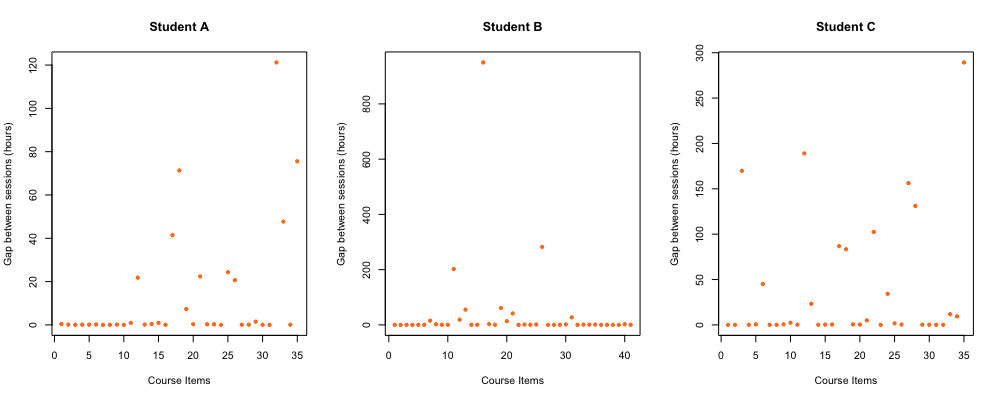
\includegraphics[scale=0.4]{sampleprogress}
    \caption{Student progress through the course Getting and Cleaning Data for three sample students. The vertical axis shows the time gap between completing an item and the next item in hours.}
    \label{figure:sampleprogress}
\end{figure}

For the average student, we can look at is the average gap between
sessions for the first and the second half of the course. We can then
calculate how much the average session gap changes from the first half
to the second. Across our sample of students who registered for the
course, the average change in session gap from the second half to the
second half is positive and equal to 132 percent. In other words the gap
between session more than doubles from the first half of the course to
the second half. Figure \ref{figure:timegapchange} shows the density
function of this statistic across our sample. The long righ tail in the
Figure supports the fact that most students follow the slowing-down
pattern. However, the Figure also shows that there are students who
speed up during the second half of the semester.

\begin{figure}[htbp]
    \centering
    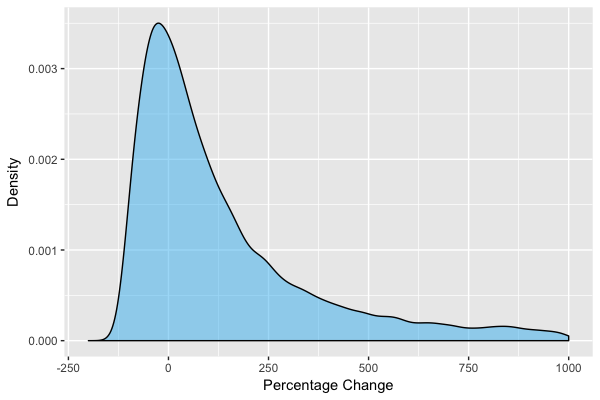
\includegraphics[scale=0.5]{timegapchange}
    \caption{Percentage change in time gaps in course progress between the first and the second half}
    \label{figure:timegapchange}
\end{figure}

We can do this analysis for some subgroups of our sample. Some of the
most interesting categories are gender, educational attainment, and
whether the learner paid for taking the course. The variable
\texttt{was\_payment} in the table
\texttt{users\_courses\_\_certificate\_payments} captures whether the
learner has ever paid for the eligibility of a course certificate,
enrolled in the course, and has not made a refund. This purchase could
be a ``single payment'' for the course or a ``bulk payment'' for a
specialization that contains the course. The following code is used for
the analysis of payers and non-payers and the results for all categories
are shown in Table \ref{tab:timecats}.

\begin{Schunk}
\begin{Sinput}
gaps.payment <- gaps %>%
    dplyr::group_by(jhu_user_id) %>%
    dplyr::summarise(avgtime = mean(time.dif)) %>%
    dplyr::inner_join(all_tables[["Getting and Cleaning Data"]][["course_grades"]],
                      by = "jhu_user_id", `copy`=TRUE) %>%
    dplyr::filter(course_passing_state_id %in% c(1, 2)) %>%
    dplyr::left_join(all_tables[["Getting and Cleaning Data"]][["users_courses__certificate_payments"]],
                     by = "jhu_user_id", `copy`=TRUE) %>%
    dplyr::filter(!is.na(was_payment)) %>%
    dplyr::group_by(was_payment) %>%
    dplyr::summarise(avggap=mean(avgtime))
\end{Sinput}
\end{Schunk}

\begin{table}
\footnotesize
\caption{Gaps between sessions for different subgropus of learners in Getting and Cleaning Data Course}\
\centering
\label{tab:timecats}
\begin{tabular}{p{3cm}|p{4cm}}
Categories & Avergae gap in hours \\
\addlinespace
\toprule
Gender & Female: 39\\
       & Male: 36\\
\midrule
Educational Attainment & Less than high school: 152\\
           & High school diploma: 39\\
           & College (no degree): 39\\
           & Associate degree: 23\\
           & Bachelor's degree: 32\\
           & Master's degree: 38\\
           & Professional degree: 22\\
           & Doctoral degree: 34\\
\midrule
Paid for the course? & Yes: 36\\
           & No: 39\\
\addlinespace
\bottomrule
\end{tabular}
\end{table}

Last exercise in our analysis is to study how Courera's change in policy
from a pay-per-course business model to a subscription model changed
students' progression throughout the course. In October 30, 2016,
Coursera introduced a new payment system through which they allowed
students to purchase access to all content in a specialization on a
month-by-month or annual basis. As a result, student would only pay for
the amount of time they need to learn the material. This system replaced
the existing model where students would pay up front for each course
regardless of how long it took them to finish the course. An interesting
exercise then is whether the switch to this system where payments is
tied to the length of time it takes students to finish the class make
students finish faster. The following code calculates the average number
of courses passed in the first week of activity for the two groups:
those who enrolled in the course before October 30, 2016 and those who
enrolled after. Our hypothesis is that those who pay monthly are more
likely to finish more items in the first week than those who pay a fixed
price.

\begin{Schunk}
\begin{Sinput}
passed.items.policy <- passed.items %>%
    dplyr::left_join(all_tables[["Getting and Cleaning Data"]][["course_memberships"]], 
                     by = "jhu_user_id", `copy`=TRUE) %>%
    dplyr::filter(!is.na(course_membership_ts)) %>%
    dplyr::mutate(subscription = ifelse(course_membership_ts < "2016-11-01 00:00:00", 
                                        "before", "after")) %>%
    dplyr::group_by(subscription) %>%
    dplyr::summarise(subnw = mean(nweek1))
\end{Sinput}
\end{Schunk}

The results suggest that those who enrolled before the policy change on
average passed three courses less than the group who enrolled after (9
versus 12). Figure \ref{figure:policy} shows the density function of the
number of passed items in the first week of activity for the two groups.
This comparison, however, has a caveat: there is some selection bias
since those who enrolled before and those who enrolled after October
2016 may be fundamentally different.

\begin{figure}[htbp]
    \centering
    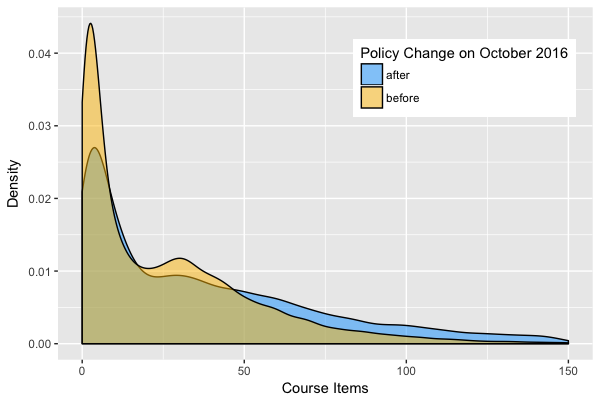
\includegraphics[scale=0.5]{policy}
    \caption{Density functions for the number of passed items in the first week of course activity for Getting and Cleaning Data for those who enrolled in the course before October 30, 2016 and those who enrolled after}
    \label{figure:policy}
\end{figure}

\subsection{Discussion}\label{discussion}

\bibliography{RJreferences}

\address{%
Aboozar Hadavand\\
Bloomberg School of Public Health, Johns Hopkins University\\
615 N. Wolfe Street\\ Baltimore, MD 21205, USA\\
}
\href{mailto:hadavand@jhu.edu}{\nolinkurl{hadavand@jhu.edu}}

\address{%
Jeffrey Leek\\
Bloomberg School of Public Health, Johns Hopkins University\\
615 N. Wolfe Street\\ Baltimore, MD 21205, USA\\
}
\href{mailto:jtleek@jhu.edu}{\nolinkurl{jtleek@jhu.edu}}

